\section{Diseño de un analizador léxico}

Se ha diseñado el analizador léxico del lenguaje mediante un diagrama de transiciones, como se observa en la figura \ref{fig:diagrama_afd}.
Éste ha sido realizado usando la herramienta \textit{JFLAP}. Hemos incluido todos los posibles síbolos que pueden haber en
el subconjunto \textit{Tiny(0)}, contando finalmente con un total de 33 estados.

\begin{figure}[H]
    \centering
    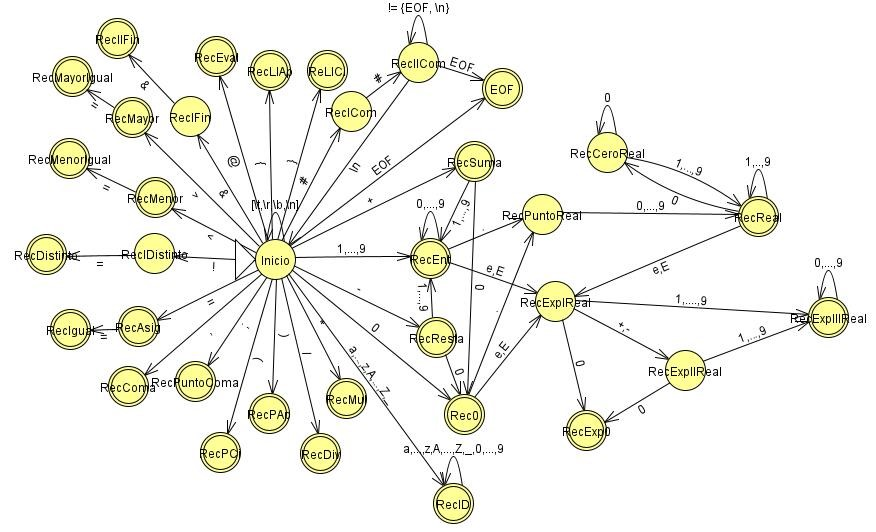
\includegraphics[width=0.8\linewidth]{Secciones/Hito1/Tiny0/diagrama_afd.jpg}
    \caption{AFD para Tiny(0)}
    \label{fig:diagrama_afd}
\end{figure}